\documentclass[main.tex]{subfiles}

\begin{document}
With the pieces in place, the fitting of the data beta spectrum can take place.
The output of the GEANT4 simulation was used for this fitting.  

\section{Fitting Method}
Four GEANT4 simulations were needed for the fit.
The simulations differed by what was given as the input spectrum for the electrons.
These are summarized in table \ref{tab:4histfit}

\begin{table}[!hbt]
	\centering
	\caption{The four histograms used for the fit}
	\resizebox{\textwidth}{!}{
		\begin{tabular}{lrr}
		Name & Formula & Normalization (in keV) \\
		f(E) & PS(E) * Corrections & 1 \\
		g(E) & PS(E) * E * Corrections & 3.35e-4 \\
		h(E) & PS(E)  * E * E * Corrections & 9.89e-8 \\
		j(E) & PS(E)/E * Corrections & 2494 
		\end{tabular}}
		\label{tab:4histfit}
\end{table}

The $E$ is the total electron energy in this case.
These pieces came from the nuclear shape factor and the Fierz term. 
The normalization is relative to f(E) before each piece was fed into GEANT4. 
Each of these pieces was generated with the same number of events in GEANT4.
Each of them was filtered as described in the previous chapter.
However, the simulations needed further processing before being used in the fit function. 
The first was applying the detector resolution

\subsection{Detector Resolution}
\label{sec:convolution}
The next step was the apply the detector resolution to this histogram.
This was done by applying a convolution function to the histograms built from the GEANT4 output files.
The convolution function was

\begin{equation}
	\sigma = A\sqrt{E}
	\label{eq:convo}
\end{equation}

where $\sigma$ was the energy resolution, $E$ the energy, and $A$ a constant found through a calibration.
This was done by looping through each of the histograms bin by bin and reading the number of counts in each bin.
For each bin a Gaussian function was built.
The centroid of the Gaussian was the center of each bin in keV.
The $\sigma$ of the Gaussian was calculated by using equation \ref{eq:convo}.
This Gaussian function was sampled as many times as there were counts in the bin.
These samples were filled into a new histogram.
This was repeated bin by bin until all bins were distributed.
This was done separately for the beta-only spectrum and the beta-gamma sum spectrum. 

\subsubsection{Determining Detector Resolution}
In order to properly fit the energy spectrum, a calibration of the CsI(Na) detector had to be done.
The calibration was used to find what the detector resolution was.
Several different energy lines were used to find the calibration and the energy resolution function.
The lines were the 1.173228 MeV and 1.332492 MeV gammas from a $^{60}$Co source, the 0.661657 MeV gamma ray from a$^{137}$Cs source, and the 0.511 MeV and 1.274527 MeV gamma rays from a $^{22}$Na source.
These gamma rays were fitting with a Gaussian and a background.
The background varied from no background, a linear background, a quadratic background, and an error function background.
For the $^{60}$Co, both peaks were fit at once.
These different background gave slightly different results for the centroids and the widths of the Gaussian.
The different widths and centroids were taken as a systematic error.
From the centroids, the calibration for each detector was calculated and shown in equation \ref{eq:cal}

\begin{equation}
	C = G * E + b
	\label{eq:cal}
\end{equation}

where $C$ is the location of the peak in ADC channels, $G$ the gain in channels/keV, and b the offset in channels.
This calibration curve was only used for the resolution determination.
The widths of the peaks were calibrated with the gain and plotted vs energy.
Then, equation \ref{eq:convo} was fit to the results in order to determine $A$.
The value of $A$ used for this procedure was 1.112 with an uncertainty of 0.008.

After applying the detector resolution, the pile-up in the detector had to be modeled.

\subsubsection{Pile-up Modeling}
Modeling the pile-up was important for the fit. 
In order to model the pile-up properly, a model of the detector pulses was needed. 
For the CsI(Na) signals, a linear rise and then an exponential decay was used.
The linear part went from 0 to 1 over 100 ns. 
The exponential piece started at 100 ns at 1 and decayed with a $\tau$ of 760 ns.
This analytic equation was scaled up or down to whatever energy was sampled.
It was then fed into a model of trapezoidal filter of PIXIE. 
The math was the same as described in the chapter on data acquisition.

This model was tuned on calibration data. 
A run was taken of $^{137}$Cs at 25000 counts per second.
A 2000 counts per second $^{137}$Cs run was used as a background and subtracted off.
Then, samples of the background-subtracted spectrum were taken up to the end of the 661 keV peak.
Monte Carlo methods were used to model the time difference between two samples.
If the two samples fell within the pile-up window, then the piled-up signal models were fed into the trapezoidal filter.
The calculated pile-up energy was saved to a histogram.
If the two samples did not fall with in the pile-up window, then they were not fed into the filter model and just filled into the histogram.
The parameters were adjusted until the generated pile-up matched the measured pile-up in the spectrum.
The results of the tuning is seen in figure \ref{fig:pileuptune}

\begin{figure}[!htb]
	\centerline{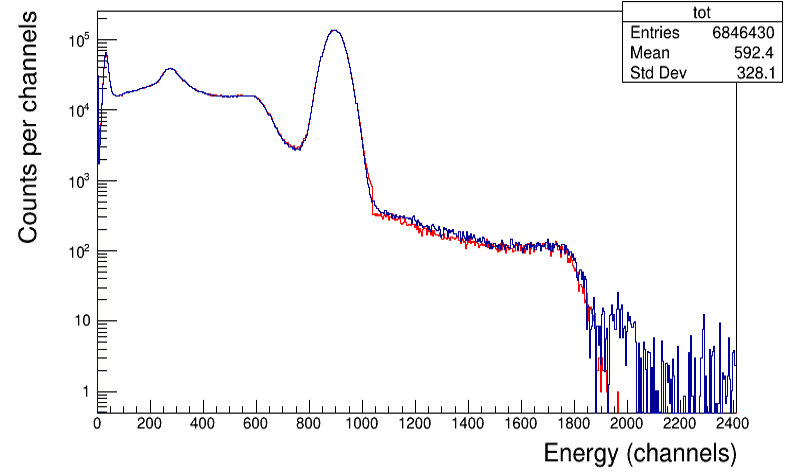
\includegraphics[width=0.78\textwidth]{PileUpTuningThesis.png}}
	\caption{The tuning of the pile-up.
		 The input spectrum is in blue.
		 It was sampled up to 1000 channels.
		 The generated spectrum is in red.}
	\label{fig:pileuptune}
\end{figure}

For the pile-up model, the resulting times are shown in table \ref{tab:tunepileupmodel}.
In addition, the parameters of the actual energy for the CsI(Na) implant detector are shown.

\begin{table}[!hbt]
	\centering
	\caption{Pile-up model parameters compared to the energy filter parameters}
	\resizebox{\textwidth}{!}{
		\begin{tabular}{lrr}
		Parameter & Pile-up model value & Energy filter value \\
		$\tau$ & 880 ns & 900 ns \\
		$tPEAKING$ & 880 ns & 480 ns \\
		$tGAP$ & 72 ns & 48 ns  
		\end{tabular}}
		\label{tab:tunepileupmodel}
\end{table}

The $\tau$ value in the pile-up tuning is very similar to that of the energy filter.
The other parameters are roughly double in the pile-up model compared to that in the PIXIE energy filter.

The pile-up model was applied to the simulation after the detector convolution was applied. 
Of the four different simulations needed for a fit, only the one with the phase space times corrections was fed into the pile-up model.
Due to the nuclear shape factor, applying the pile-up to the other terms would be a correction to a correction. 
The beta only spectrum and the beta-gamma sum spectrum of this simulation was added together and fed through the pile-up model.
With all the pieces in place, the fit function can be described. 

\subsection{Fit Function}
For the fit function, the convoluted histograms and pile-up were rebinned to a bin width of 64 keV.
Then, each of the histograms were turned into a spline. 
The five splines were fed into a fit function.
The fit function is shown in equation \ref{eq:betafit}

\begin{equation}
	H(E) = A * (( 1 + C_{0}) f(E) + C_{1}g(E) + C_{2} h(E) + (C_{-1} + b_{gt} m_{e}) j(E)) + B * pu(E)
	\label{eq:betafit}
\end{equation}
    
where $A$ is the normalization, $B$ the level of pile-up, $pu(E)$ is the generated pileup spectrum, $E$ the kinetic energy of the electron, the $C$s are the piece of the shape factor as defined in equation \ref{eq:shapefactor},  $b_{gt}$ is the Fierz term, $m_{e}$ the electron mass, and $f(E),g(E),h(E),$ and $j(E)$ the different simulation results as shown in table \ref{tab:4histfit}.
In order to change the units of the x-axis in the data to energy in keV, a calibration was needed.
For this calibration, the offset was fixed in the fit function.
However, the gain of the calibration was left as a free parameter.
This was to account for gain shifts, such as an apparent rate-dependent gain shift due to the afterglow in the crystal.

In the fit, each of the $C$s were written out in terms of the nuclear form factors.
In these form factors, $b_{wm}$ was left as a potential free parameter. 
If $b_{wm}$ was fit with the fit function, $b_{gt}$ was fixed to be 0. 
If $b_{gt}$ was fit, then $b_{wm}$ was fixed to be 43.4. 
In total, the fit function had four free parameters:
$A$, $B$, the gain, and either $b_{wm}$ or $b_{gt}$. 

In order to benchmark this fitting method, pseudo-data was generated and fit.


\subsection{Fit Method Characterization}
Different methods of the fit function were tested. 
The first is the so-called "hybrid method", where only one simulation is needed.
The GEANT4 with only the phase space and corrections is generated. 
Then, it is multiplied by the shape factor, as shown in equation \ref{eq:hybridmodel}

\begin{equation}
	H(E) = A * f(E) * S(E)
	\label{eq:hybridmodel}
\end{equation}

with $A$ being a normalization constant, $f(E)$ being the simulation with the detector resolution applied, and $S(E)$ the shape factor. 
This method of fitting is not completely correct, as the $E$ in $f(E)$ is not the same as the initial energy in the shape factor $S(E)$. 

The first test was done just with a linear term in the psuedo-data.
An older version of the GEANT4 code had a phase space times corrections times a linear shape factor fed into it.
This psuedo-data was fit with the hybrid model.
Initially, the shape factor was applied to total energy inside the implant detector.
This was found to induce a shift of the measured linear term.
Applying the shape factor only to the beta only part of the spectrum solved this issue. 

To further test this method, simulated data was used. 
One had had the nuclear shape factor with $b_{wm} = 43.4$.  
The other had no shape factor.
After applying the coincidence condition to both of these simulations, the function with no shape factor was used to fit the function with the shape factor. 
The gain in these fits was left as a free parameter, and the offset was fixed to a value of 0. 
The spectrum with the shape factor became the pseudo-data spectrum.
To manually check the statistical uncertainty, the pseudo-data spectrum was fluctuated.
Each bin had its content and error read. 
That bin error and content was used to build a Gaussian random number distribution.
This random number distribution was sampled, and a new bin center created.
After doing this to the entire spectrum, the new spectrum was fit.
The resulting $b_{wm}$ was recorded.
Then, $b_{wm}$ was set to 43.4, and the Fierz term fit. 
These fitted terms were saved to a histogram.
This was done 1000 times to get a spread of values.
From this, it was discovered that spline interpolation was the best way to fit the spectra.

The same method was used to see if the fitting method induced a lower beta cut effect or not. 
1000 spectra were generated by scrambling one spectrum over and over.
These spectra were fit from a lower beta cut up to the end point minus 100 keV.
The lower beta cut was varied from 200 keV up to 2 MeV.
From this it was found that this fitting method induced an effect above 1200 keV.
This effect was very large in the measurement of $b_{gt}$.

Doing the same thing with the four-histogram fitting method shown above showed that there is not such a large lower beta cut effect.
The four histogram fit is the one described above. 
More pseudo-data was generated, along with four histograms to be used for fitting.
This was largely done to get a handle of the normalization of the histograms.
The normalization was obtained by taking the ratios of the histograms and fitting them with the functional forms. 
After the normalization, the fit was done.
The output $b_{gt}$ and $b_{wm}$ obtained was the one put in.

\section{Experimental Data Processing}
After the fitting method was tested and verified, the data was ready to be fit 
For the fit, the experimental data had to be processed as well. 
The data was put in coincidence much like in the half-life measurement.
The energy spectrum of the implant detector was put in coincidence with the 4 gamma detectors.
The energy cuts of the gamma detectors were the same as in the life-time measurement.
An additional condition was that only one of the gamma detectors could have fired for each event.
This conditions was mirrored in the GEANT4 as well.

An additional condition in the data was a time difference condition.
For this measurement, the time difference between a beta event and a gamma event had to be between -300 and 24 ns.
This captures the entire spectrum, as the time stamps show a large energy dependence. 
Then, a 2-D histogram was built, with energy on one axis and time since last beam on on there other.
The decay cycles were 22 seconds long for the CsI(Na) implant data. 
The decay cycles were split up into 3 segments with equal number of counts.
To do this, it was assumed that the rate depended on the time as an exponential.
This exponential had a half-life of 11 seconds.
The time interval was split in such a way that the integral of the exponential was equal over 3 different segments.
The total time interval was from 1.5 to 22 seconds.
These splits worked out to be at 5.89 s and at 11.98 seconds. 
This 2-D histogram was projected onto the time axis between the splits in order to build the energy spectrum of the fit. 

After processing the data, the fit was done run by run.
First a prefit for each section was done to calibrate the energy from 500 channels to 6000 channels.
This was done to obtain a calibration of the data.
Then, two endpoints fixed in keV were used for the actual fit.
The fitting function with a fixed offset was fit using a maximum likelihood method.
The resulting $b_{wm}$ was recorded.
For the Fierz term fit, the $b_{wm}$ of $^{20}$F decay (43.4) was applied to the shape factor.
The fit was done again and the $b_{gt}$ was recorded.

The offset used for the fit was varied.
The effect of the offset will be discussed in the next section. 
The calibrated end points were 250 keV to 7500 keV. 
A sample fit is shown in figure \ref{fig:samplefit}, where the offset was fixed to 0.

\begin{figure}[!htb]
	\centerline{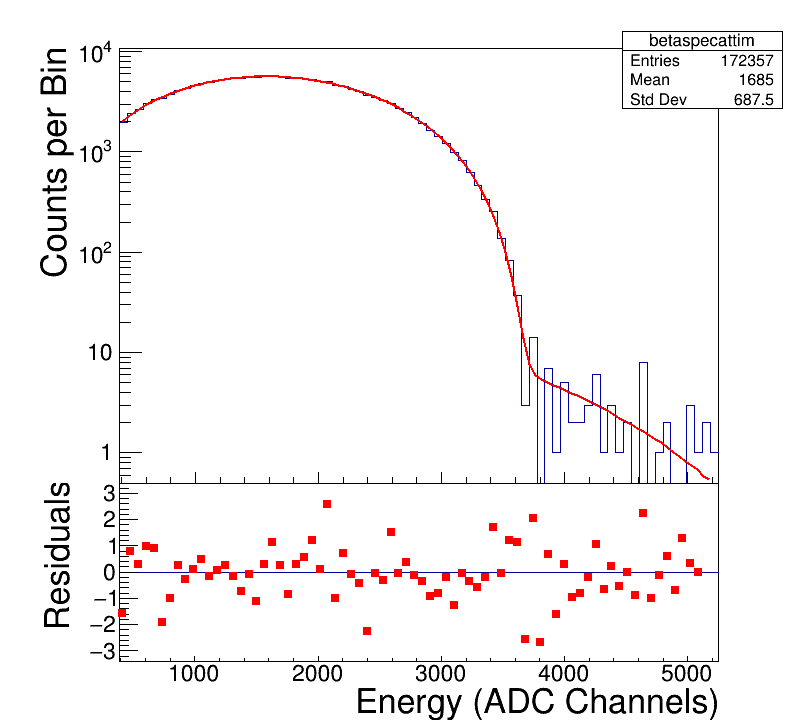
\includegraphics[width=0.78\textwidth]{CsIRun317FierzTermResids.png}}
	\caption{A sample fit of the beta spectrum. 
		 The residuals of the fit are shown below the graph}
	\label{fig:samplefit}
\end{figure}

\section{Systematic effects}

After testing the fit and fitting the data, the systematic effects were investigated.
These mostly stem from the inputs to the GEANT4 simulations or inputs to the fits.
The largest effect had to do with where the fit was started.

\subsection{Lower Beta Cut Effect}

The lower beta cut effect is the systematic shift of both the $b_{wm}$ and $b_{gt}$ as a function of where the fit started.
There are several different inputs that can induce such an effect.

\subsubsection{The Offset}
Initially, the offset used was the offset from the calibration  in equation \label{eq:cal}.
The offset used was 10.05 ADC units.
This calibration was determined using photons instead of electrons.
%Electrons generate 2\% less light than photons \cite{REFHERE} % maybe knoll?
This means that the offset found from this fit is suspect to apply to our electron shape measurement.

When applying an offset of 10.05 in a fit of the data, it was found that the output varied greatly as a function of where the fit was started.
The effect in $b_{wm}$ and $b_{gt}$ is shown in figure \ref{fig:offset10LBCeffect}.

\begin{figure}
    \centering
    \begin{minipage}{0.50\textwidth}
        \centerline{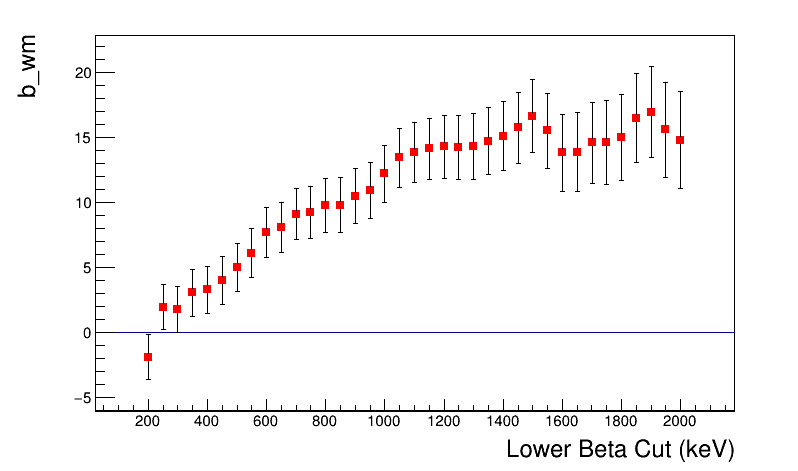
\includegraphics[width=0.9\textwidth]{CsILBCvbwmOffsetis10p054histfit.png}}
    \end{minipage}\hfill
    \begin{minipage}{0.50\textwidth}
        \centerline{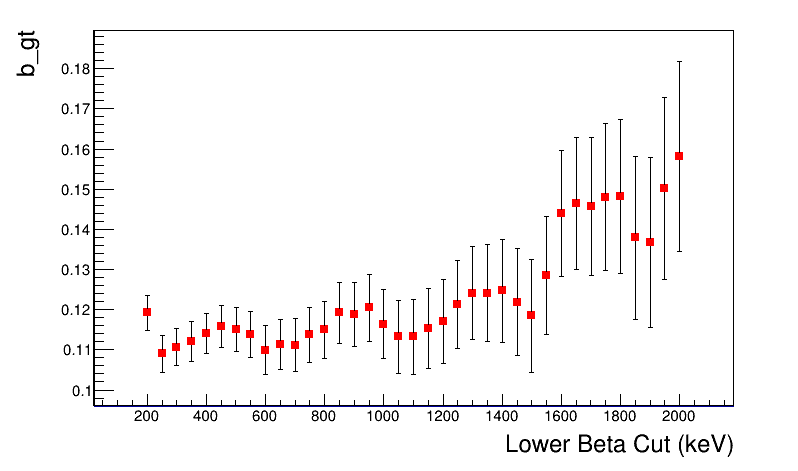
\includegraphics[width=0.9\textwidth]{CsILBCvbgtOffsetis10p054histfit.png}}
    \end{minipage}
    \caption{The depedence of the parameters to the start of the fit.
	     The offset here is 10.05.}
    \label{fig:offset10LBCeffect}
\end{figure}

To test the effect of the offset, a Monte Carlo was written.
A sample histogram with only the phase space and the shape factor was generated. 
These histograms were generated with an offset of 10 ADC units.
A random gain was applied to the psuedo-data histogram. 
Then, the fit function had a different offset applied to it.
For example, fitting the histogram generated with an offset of 10, and fit with an offset of 20 gives an effect as seen in \ref{fig:MCoffset10applied20}.

\begin{figure}
	\centerline{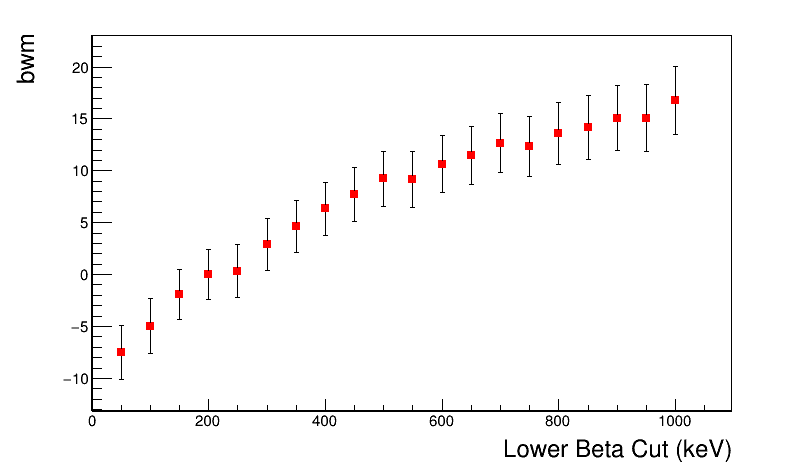
\includegraphics[width=0.9\textwidth]{MCLBCvbwmOffsetis10Applied20.png}}
	\caption{The effect of the lower beta cut in a simulation when the applied offset is 10 units higher than the real offset.}
	\label{fig:MCoffset10applied20}
\end{figure}

This effect can be exploited to determine an offset using only the data. 
The size of the slope induced is linear compared to the offset.
By adjusting the offset and noting the slope of the $b_{wm}$ vs the lower beta cut and plotting against the offset, the location of zero slope can be calculated.
This was done, and the result is seen in figure \ref{fig:offset0LBCeffect}.

\begin{figure}
    \centering
    \begin{minipage}{0.50\textwidth}
        \centerline{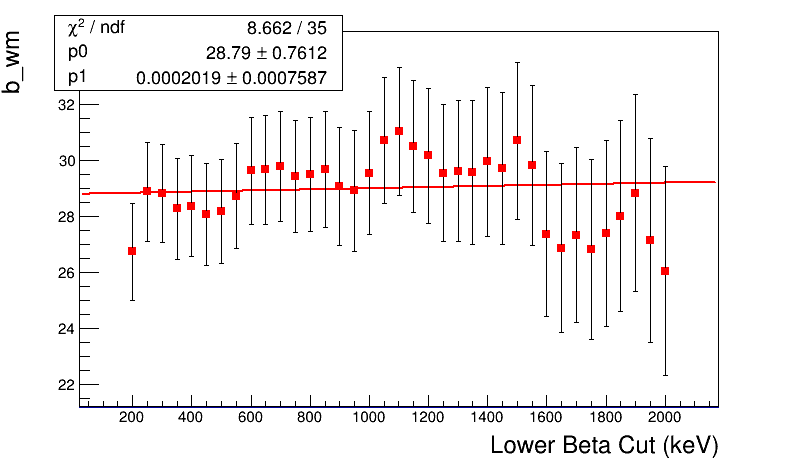
\includegraphics[width=0.9\textwidth]{CsIbwmvLBCDrawingGeo_OffsetisZero.png}}
    \end{minipage}\hfill
    \begin{minipage}{0.50\textwidth}
        \centerline{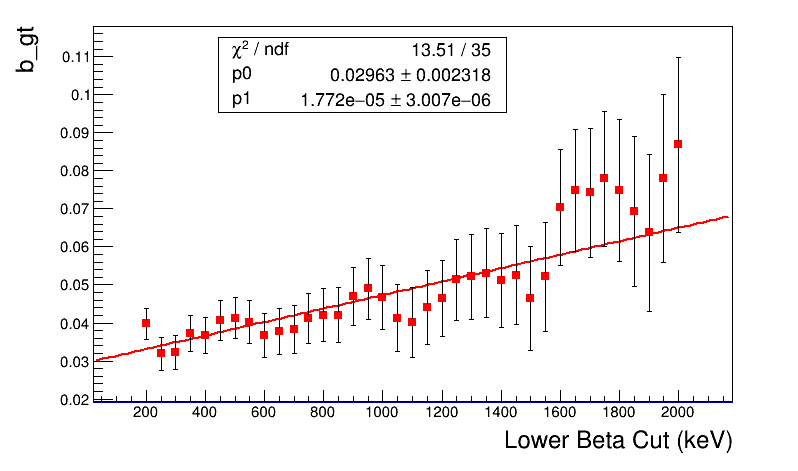
\includegraphics[width=0.9\textwidth]{CsIbgtvLBCDrawingGeo_OffsetisZero.png}}
    \end{minipage}
    \caption{The depedence of the parameters to the start of the fit.
	     The offset here is 0.
	     The $b_{wm}$ is independent of the start of the fit, but the $b_{gt}$ still has a large effect}
    \label{fig:offset0LBCeffect}
\end{figure}


Doing this procedure gives an offset that depends on the input geometry of the GEANT4 simulation.
As seen in figure \ref{fig:offset0LBCeffect}, the $b_{gt}$ still depends greatly on where the fit starts.
Other effects are important. 

\subsubsection{The Relative Normalization of the Beta-gamma Sum Spectrum}

The output of the GEANT4 Monte Carlo was processed into two different parts.
The two parts were summed with a factor of 1 in front of the beta-gamma sum spectrum in figure \ref{fig:offset0LBCeffect}.
This relative normalization is given from GEANT4.
Using the same Monte Carlo, this factor was adjusted in the psuedo-data and the fitting functions.
It was found that an effect as seen in the data can be produced by multiplying the beta-gamma sum spectrum in both the data and the fit function induced a shift very similar to that in figure \ref{fig:offset0LBCeffect}.
This is seen in figure \ref{fig:MCTimes5}.    

\begin{figure}
    \centering
    \begin{minipage}{0.50\textwidth}
        \centerline{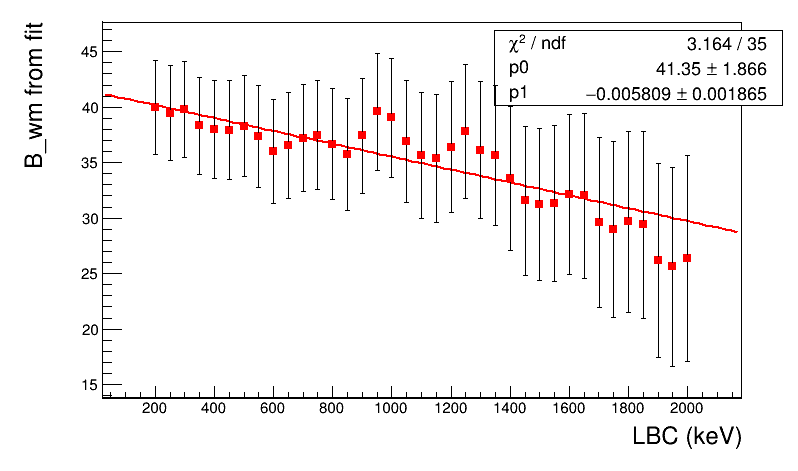
\includegraphics[width=0.9\textwidth]{MCbwmvLBC_BGBothTimes5.png}}
    \end{minipage}\hfill
    \begin{minipage}{0.50\textwidth}
        \centerline{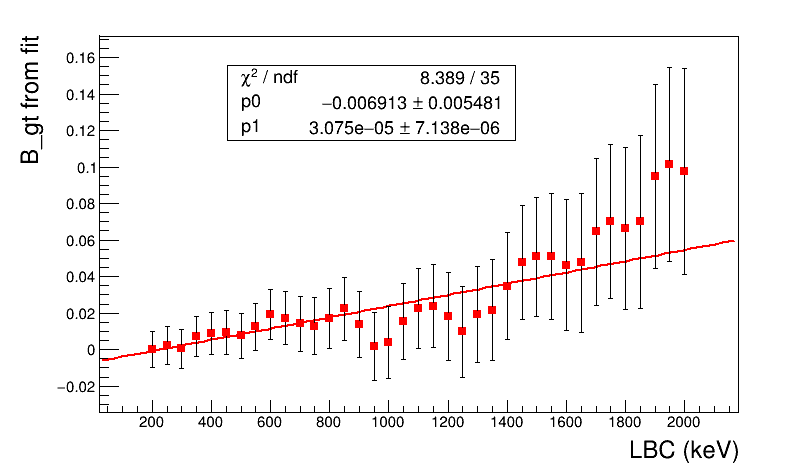
\includegraphics[width=0.9\textwidth]{MCbgtvLBC_BGBothTimes5.png}}
    \end{minipage}
    \caption{Monte Carlo data with a LBC effect due to the beta-gamma sum spectrum}
    \label{fig:MCTimes5}
\end{figure}

This is odd, as the fit function and the psuedo-data function have the same values.
The input values of the $b_{wm}$ and $b_{gt}$ can be recovered by this fit.
However, to do this, the offset in the fit function is set to 8.6 ADC units.
The sum spectra in each of the 4 hists is increased to 3.8 times that of output of the Monte Carlo.
These two parameters are unphysical.
The input offset was 0 and the input background level was 5.

Adjusting the level of the beta-gamma sum spectrum affects the $b_{gt}$ more than the $b_{wm}$.
This parameter can be adjusted to make the $b_{gt}$ indepedent of the start of the fit in figure \ref{fig:offset0LBCeffect}. 
This gives the results in figure \ref{fig:dataoffset0BG10per}. 

\begin{figure}
    \centering
    \begin{minipage}{0.50\textwidth}
        \centerline{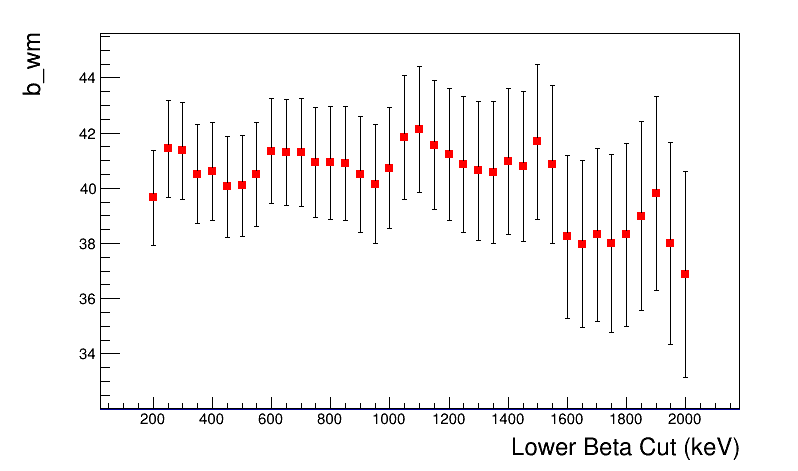
\includegraphics[width=0.9\textwidth]{CsIbwmvLBCDrawingGeo_OffsetisZero_BGis10percent.png}}
    \end{minipage}\hfill
    \begin{minipage}{0.50\textwidth}
        \centerline{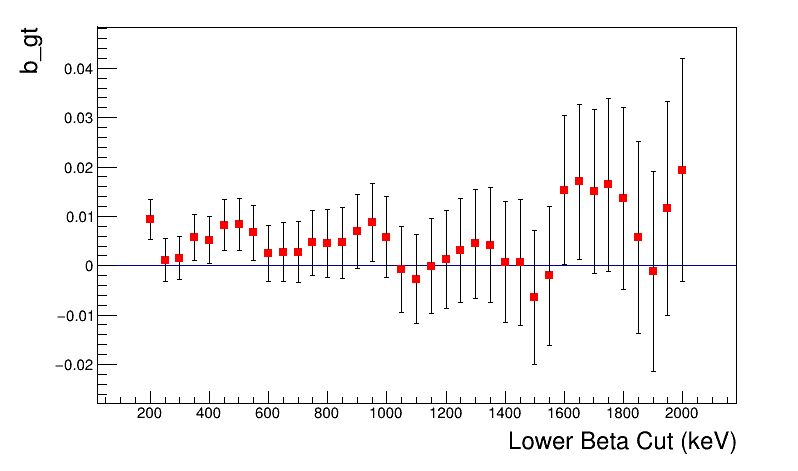
\includegraphics[width=0.9\textwidth]{CsIbgtvLBCDrawingGeo_OffsetisZero_BGis10percent.png}}
    \end{minipage}
    \caption{Adjusting the beta-gamma sum spectrum level to flatten out the $b_{gt}$}
    \label{fig:dataoffset0BG10per}
\end{figure}

However, to obtain these results, the level of the beta-gamma sum spectrum must be set to 0.096. 
It is unlikely that the GEANT4 Monte Carlo is that far off, and that this number corresponds to anything physical.
It is unclear if this procedure is a valid one to take.

\subsubsection{The Convolution}

Another potential effect is if the detector resolution was applied incorrectly.
To test that, a Monte Carlo simulation was written.
The space space in equation \ref{eq:phase_space} was multiplied by the shape factor in equation \ref{eq:shapefactor}.
This function was sampled $10^{9}$ times twice to build two histograms. 
Both histograms had a detector resolution applied as described in section \ref{sec:convolution}
One histogram was sampled a further $10^{6}$ times 10 times to build a sample data set.
The other convoluted histogram was used to fit the generated data set.
The first histogram's $A$ was fixed, while the second histogram's $A$ was adjusted.
When the sample data's $A$ matched the $A$ that were used, no dependence of $b_{wm}$ on the start of the fit.
When the $A$ of the data sample and the $A$, the first thing that happened was that the $b_{wm}$ changed.
If the $A$ differ by a factor of 2 or more, a shift in $b_{wm}$ appears.
However, this is much larger than any uncertainty in detector resolution.
The effect of a wrong detector resolution is negligible. 

\subsection{Other Systematic Effects}

The lower beta cut effect is the largest of the systematic effects.
A summary of the other systematic effects is shown in table \ref{tab:systeffects}.
These are indepedent on the lower beta cut and other input parameters to the fit.

 

\end{document}
